% !TeX program = lualatex
% !BIB program = bibtex
% Auriga theme
% https://github.com/anishathalye/auriga

\documentclass[14pt,aspectratio=169]{beamer}
\usepackage{pgfpages}
\usepackage{fancyvrb}
\usepackage{tikz}
\usepackage{pgfplots}

\usepackage[style=authortitle,backend=bibtex]{biblatex}
\addbibresource{../Paper/references.bib}
\addbibresource{../NonlinearBiquad/Paper/references.bib}
\addbibresource{references.bib}

% \ifnotes
% \setbeamertemplate{note page}[plain]
% \setbeameroption{show notes on second screen=right}
% \fi

\usetheme{auriga}
\usecolortheme{auriga}

% define some colors for a consistent theme across slides
\definecolor{red}{RGB}{181, 23, 0}
\definecolor{blue}{RGB}{0, 118, 186}
\definecolor{gray}{RGB}{146, 146, 146}

\title{Complex Nonlinearities for Audio Signal Processing}

\author{Jatin Chowdhury}

\institute[shortinst]{Center for Computer Research in Music and Acoustics (CCRMA)}

\begin{document}

{
  % rather than use the frame options [noframenumbering,plain], we make the
  % color match, so that the indicated page numbers match PDF page numbers
  \setbeamercolor{page number in head/foot}{fg=background canvas.bg}
  \begin{frame}
    \titlepage
  \end{frame}
}

\begin{frame}{Thanks}
    \begin{itemize}
        \setlength\itemsep{1em}
        \item Julius Smith
        \item Dave Berners
        \item Viraga Perera
        \item GASP
    \end{itemize}
\end{frame}

\begin{frame}{Motivation}
    Flashback to 2016\dots

    \vspace{6ex}

    \begin{center}
        Trying to make a distortion effect\dots
    \end{center}
\end{frame}

\begin{frame}{Motivation}
    \begin{columns}
        \begin{column}{0.5\linewidth}
            Static Nonlinearities
            \begin{figure}
                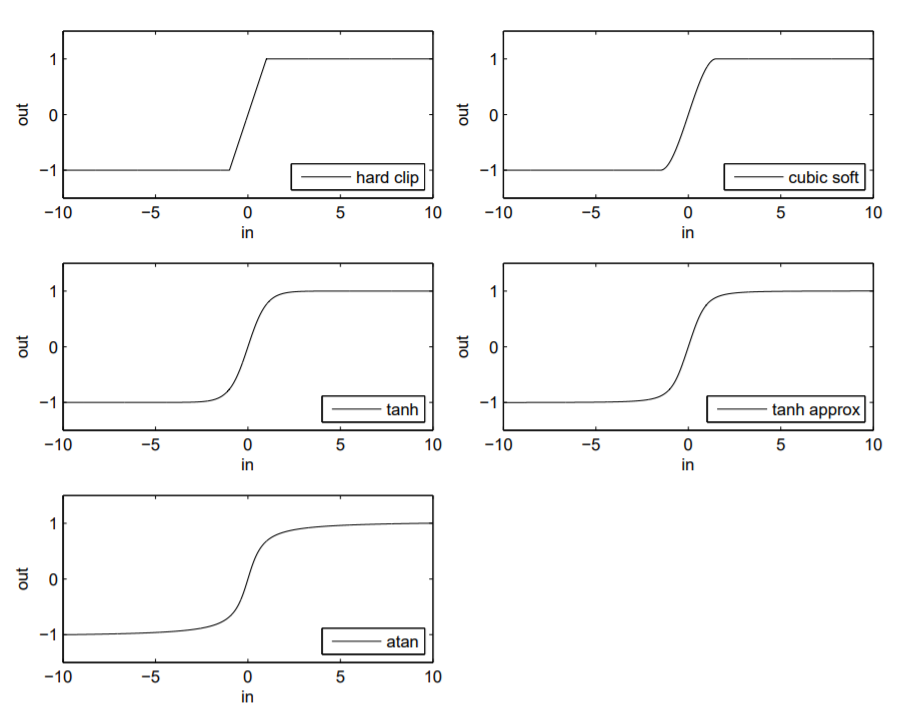
\includegraphics[height=2in]{Figures/yeh_NLs}
            \end{figure}
        \end{column}
        \begin{column}{0.5\linewidth}
            Circuit Modelling
            \begin{figure}
                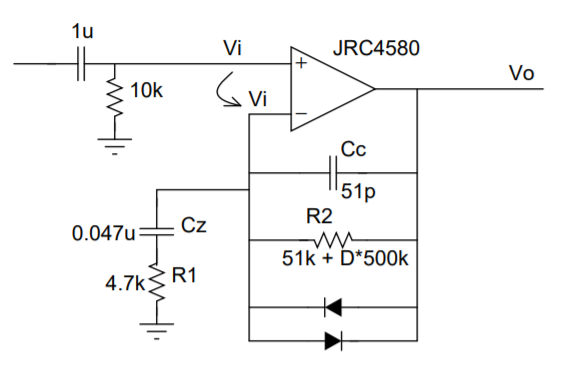
\includegraphics[width=2.5in]{Figures/yeh_pedal}
            \end{figure}
        \end{column}
    \end{columns}
\end{frame}

\begin{frame}{Motivation}
    Solution: $\tanh$ approximation \footcite{Yeh}
    \begin{equation}
        f(x) = \frac{x}{(1 + |x|^n)^{1/n}}, \quad n=2.5
    \end{equation}
\end{frame}

\begin{frame}{Motivation}
    Trying to fill the gap between:
    \newline
    \begin{itemize}
        \item Simple static nonlinear systems
        \item Physically modelled nonlinear systems
    \end{itemize}
\end{frame}

\begin{frame}{Outline}
    \begin{itemize}
        \item Basics of nonlinear signal processing
        \item Complex nonlinearities
        \begin{itemize}
            \item Double Soft Clipper
            \item Exciter
            \item Hysteresis
            \item Nonlinear biquad filters
            \item Wavefolding
            % \item Nonlinear Allpass
            \item Gated Recurrent Distortion
        \end{itemize}
    \end{itemize}
\end{frame}

\begin{frame}
    \begin{centering}
        \vskip5ex plus 1filll
        {\usebeamerfont{title page title}\usebeamercolor[fg]{title page} Building Blocks\\[1.5ex]}
        \vskip0pt plus 1filll
    \end{centering}
\end{frame}

\begin{frame}{What is a nonlinear system?}
    Frequency domain: you get out more than what you put in
    \begin{figure}
        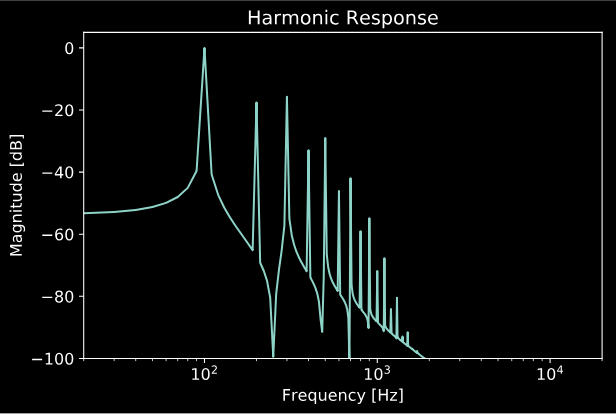
\includegraphics[width=3.75in]{../Exciter/Pics/exciter_harm.png}
    \end{figure}
\end{frame}

\begin{frame}{What is a nonlinear system?}
    Time domain: static response
    \begin{figure}
        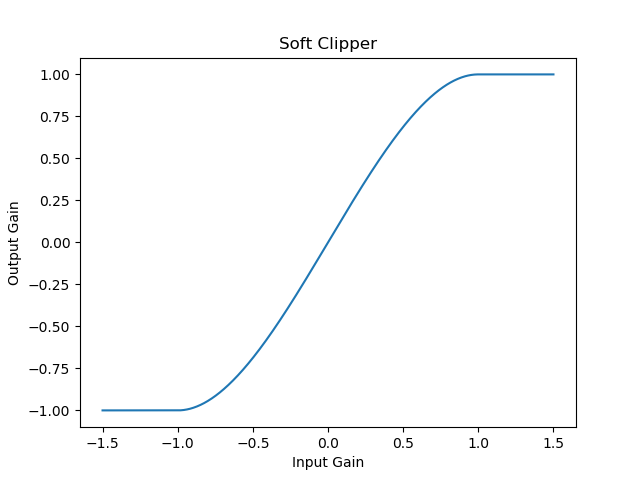
\includegraphics[height=2.5in]{../DoubleSoftClipper/Pics/SC.png}
    \end{figure}
\end{frame}

\begin{frame}{What is a nonlinear system?}
    Time domain: dynamic response
    \begin{figure}
        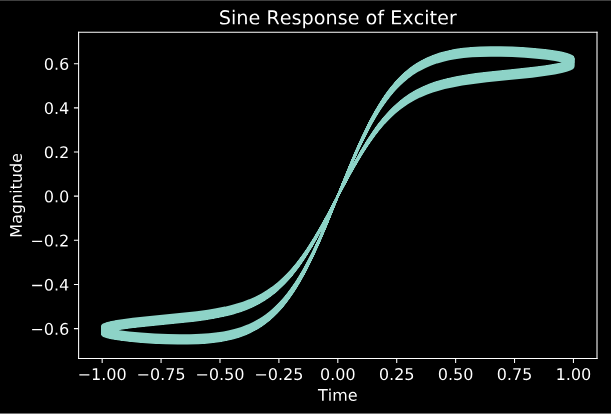
\includegraphics[width=3.75in]{../Exciter/Pics/exciter_static.png}
    \end{figure}
\end{frame}

\begin{frame}{Saturating Nonlinearities}
    \begin{figure}
        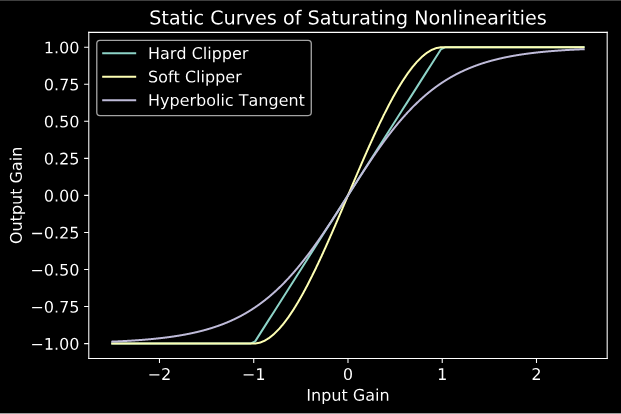
\includegraphics[width=3.75in]{../Exciter/Pics/saturating_static.png}
    \end{figure}
\end{frame}

\begin{frame}{Rectifying Nonlinearities}
    \begin{figure}
        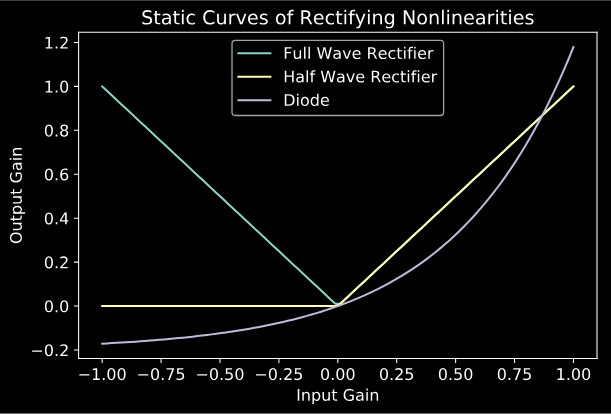
\includegraphics[width=3.75in]{../Exciter/Pics/rect_static.png}
    \end{figure}
\end{frame}

\begin{frame}{Dropout Nonlinearities}
    \begin{figure}
        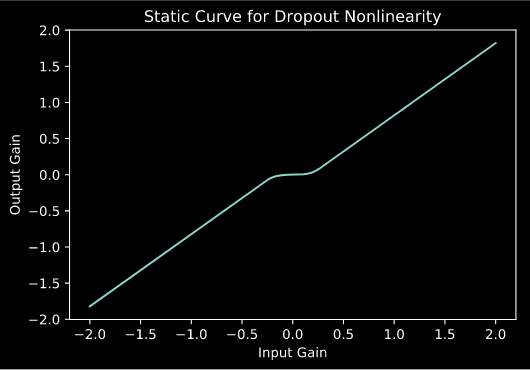
\includegraphics[width=3.5in]{../Paper/Pics/dropout.png}
    \end{figure}

    \begin{center}
        \scriptsize (also called ``dead-zone'')
    \end{center}
\end{frame}

\begin{frame}{What is a ``Complex Nonlinearity''}
    Has one of the following properties:\newline
    \begin{itemize}
        \item Is not memoryless (has some memory of past states)
        \item Has an interesting harmonic response
        \item Has interesting parameters
    \end{itemize}
\end{frame}

\begin{frame}
    \begin{centering}
        \vskip5ex plus 1filll
        {\usebeamerfont{title page title}\usebeamercolor[fg]{title page} Double Soft Clipper\\[1.5ex]}
        \vskip0pt plus 1filll
    \end{centering}
\end{frame}

\begin{frame}{Double Soft Clipper: Inspiration}
    Measured speaker response
    \begin{figure}
        \centering
        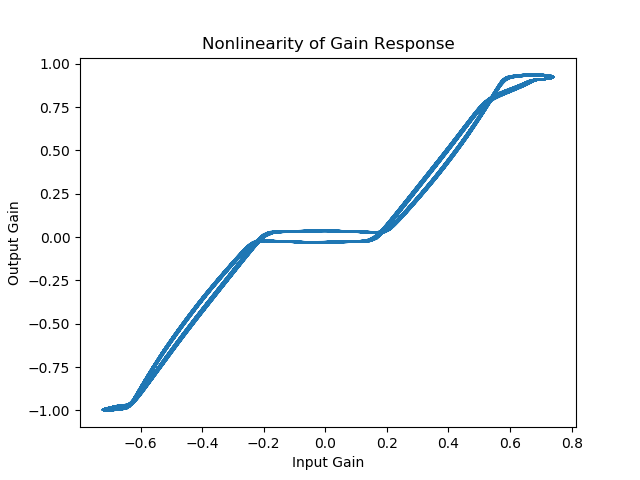
\includegraphics[height=2.5in]{../DoubleSoftClipper/Gain_Nonlinearity.png}
    \end{figure}
\end{frame}

\begin{frame}{Double Soft Clipper}
    \begin{figure}
        \centering
        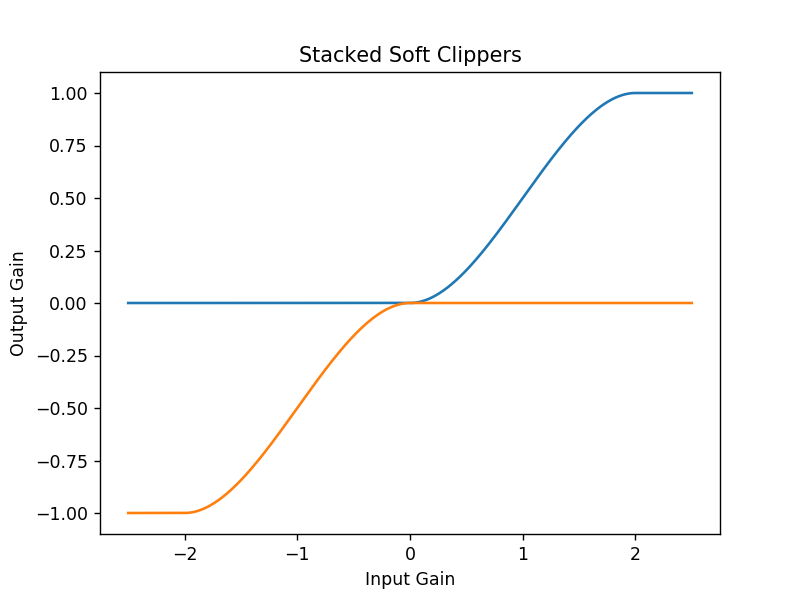
\includegraphics[height=2.5in]{../DoubleSoftClipper/Pics/stacked.png}
    \end{figure}
\end{frame}

\begin{frame}{Double Soft Clipper: Original Soft Clipper}
    \begin{equation}
        f_{SC}(x) = \begin{cases} 1 & x \geq 1 \\ \frac{3}{2} (x - x^3/3) & -1 < x < 1 \\ -1 & x \leq -1 \end{cases}
    \end{equation}
\end{frame}

\begin{frame}{Double Soft Clipper}
    \begin{equation}
        f_{DSC}(x) = \begin{cases} 1 & u \geq 1 \\ \frac{3}{4} (u - u^3/3) + 0.5 & 0 < u < 1 \\ \frac{3}{4} (u - u^3/3) - 0.5 & -1 < u < 0 \\ -1 & u \leq -1 \end{cases}
    \end{equation}
    \vspace{2ex}
    \begin{equation}
        u(x) = \begin{cases} x - 0.5 & x > 0 \\ x + 0.5 & x < 0 \end{cases}
    \end{equation}
\end{frame}

\begin{frame}{Double Soft Clipper}
    \begin{figure}
        \centering
        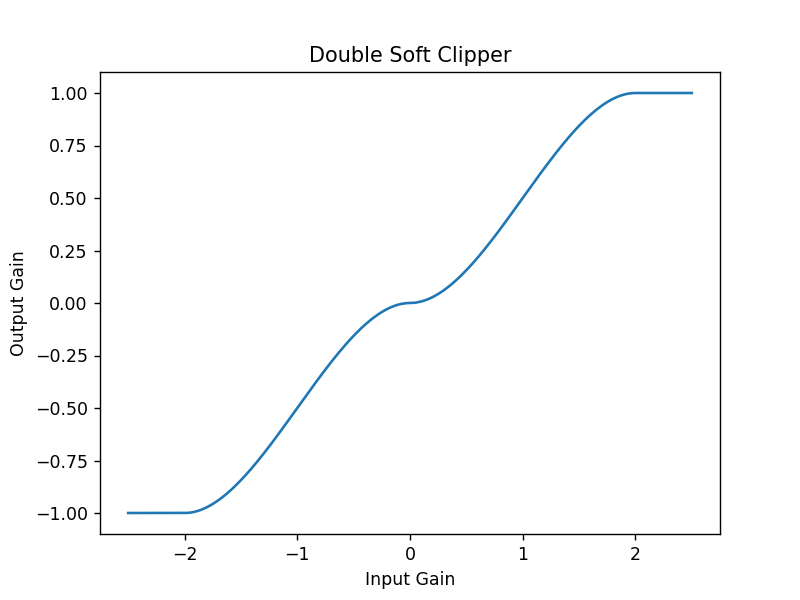
\includegraphics[height=2.5in]{../DoubleSoftClipper/Pics/Double.png}
    \end{figure}
\end{frame}

\begin{frame}{Double Soft Clipper: Parameters}
    \begin{figure}
        \centering
        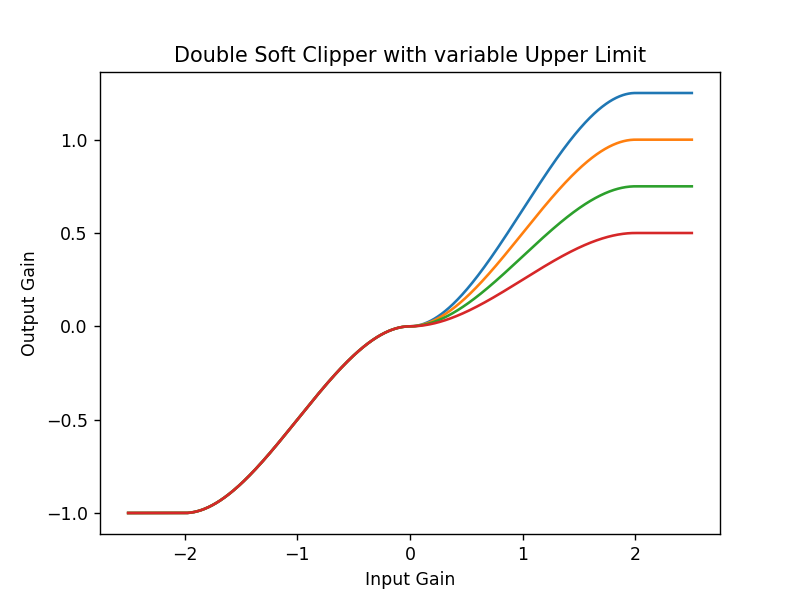
\includegraphics[height=2.5in]{../DoubleSoftClipper/Pics/VarUpperLim.png}
    \end{figure}
\end{frame}

\begin{frame}{Double Soft Clipper: Parameters}
    \begin{figure}
        \centering
        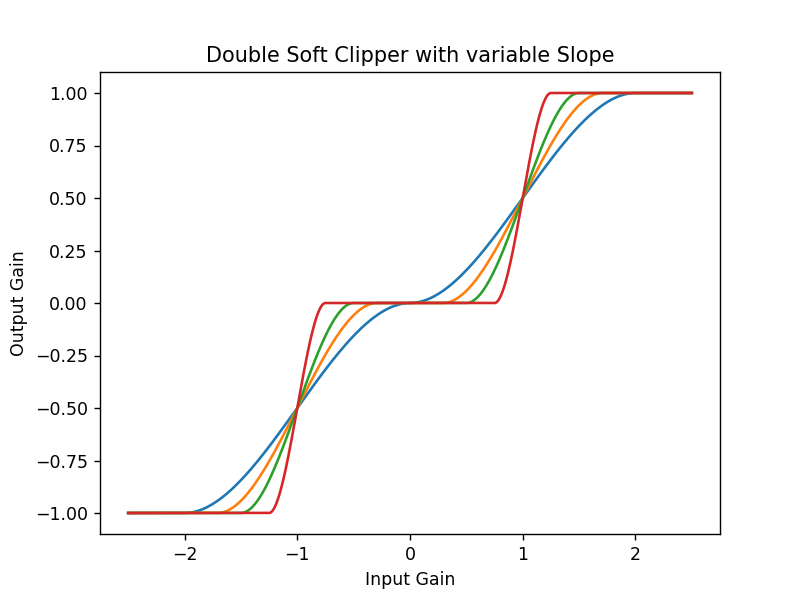
\includegraphics[height=2.5in]{../DoubleSoftClipper/Pics/VarSlope.png}
    \end{figure}
\end{frame}

\begin{frame}{Double Soft Clipper: Parameters}
    \begin{figure}
        \centering
        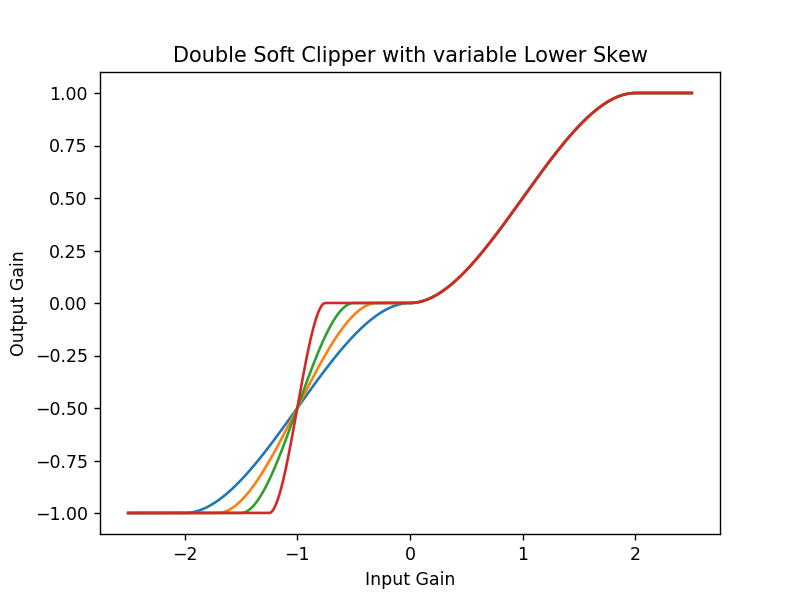
\includegraphics[height=2.5in]{../DoubleSoftClipper/Pics/VarLowSkew.png}
    \end{figure}
\end{frame}

\begin{frame}{Double Soft Clipper: Parameters}
    \begin{figure}
        \centering
        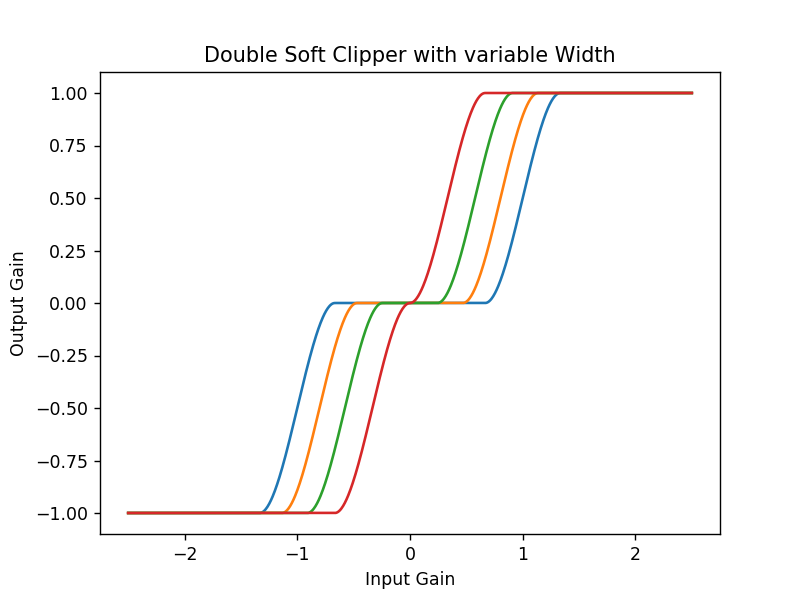
\includegraphics[height=2.5in]{../DoubleSoftClipper/Pics/VarWidth.png}
    \end{figure}
\end{frame}

\begin{frame}{Double Soft Clipper: Weird}
    \begin{figure}
        \centering
        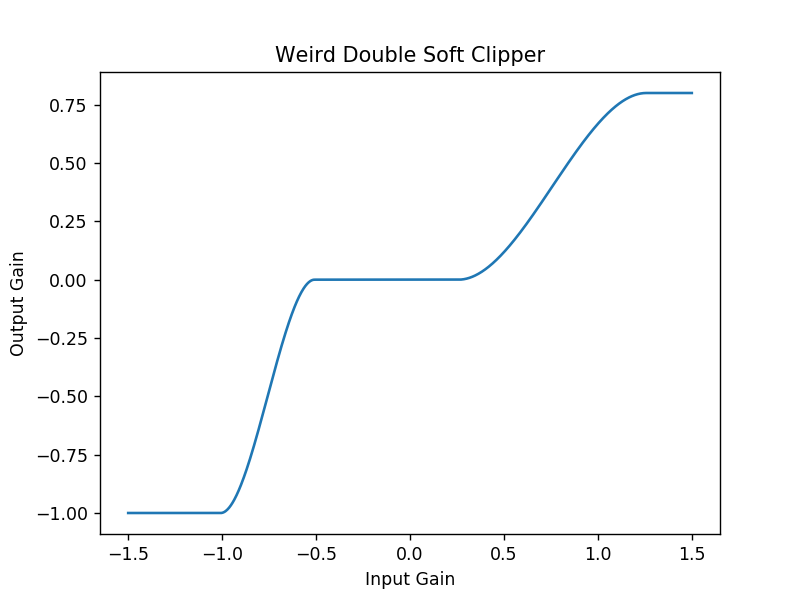
\includegraphics[height=2.5in]{../DoubleSoftClipper/Pics/Weird.png}
    \end{figure}
\end{frame}

\begin{frame}{Double Soft Clipper: Harmonic Response}
    \begin{figure}
        \centering
        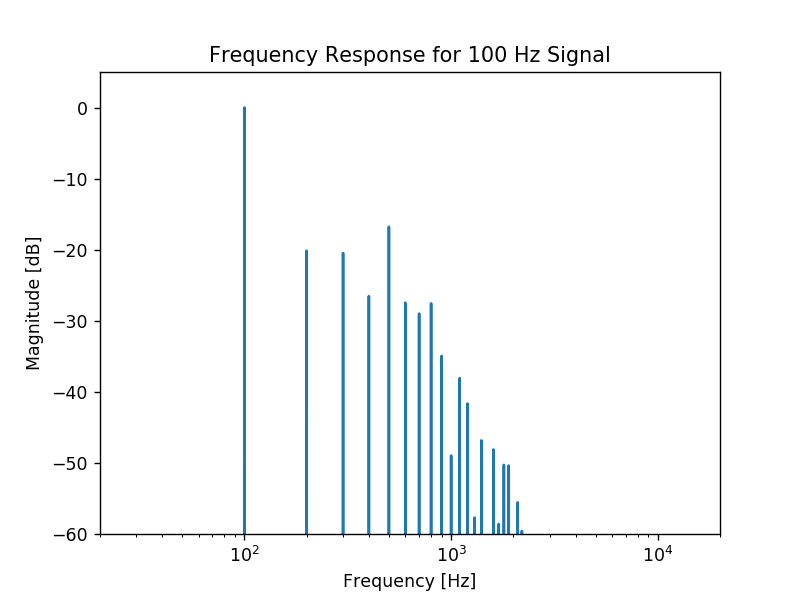
\includegraphics[height=2.5in]{../DoubleSoftClipper/Pics/Freq.png}
    \end{figure}
\end{frame}

\begin{frame}
    \begin{centering}
        \vskip5ex plus 1filll
        {\usebeamerfont{title page title}\usebeamercolor[fg]{title page} Harmonic Exciter\\[1.5ex]}
        \vskip0pt plus 1filll
    \end{centering}
\end{frame}

\begin{frame}{Harmonic Exciter}
    What is a harmonic exciter?\vspace{3ex}
    \begin{itemize}
        \item Add subtle harmonic distortion
        \item Make audio sound ``shiny'', ``brighter'', ``enhanced''
        \item Used for mixing, live broadcasts,
        restoring old recordings with missing spectral content
    \end{itemize}
\end{frame}

\begin{frame}{Aphex Aural Exciter\footcite{aphex}}
    \begin{figure}
        \centering
        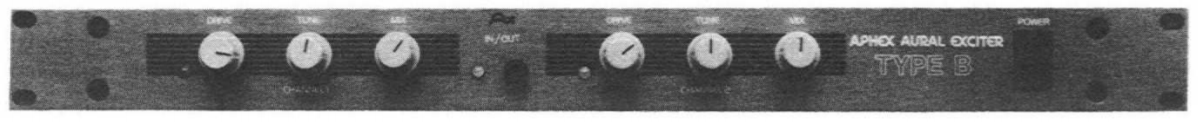
\includegraphics[width=4.25in]{Figures/aphex.png}
    \end{figure}
    \begin{itemize}
        \item Introduced in the mid-1970's
        \item Used by Jackson Browne, The Four Seasons, Linda Ronstadt, and more
        \item Originally rented to studios for \textbf{\$30 per minute}
    \end{itemize}
\end{frame}

\begin{frame}{Harmonic Exciter}
    Goals:
    \vspace{3ex}
    \begin{itemize}
        \item Exciter model that sounds ``smooth''
        \item Generalize the model to transcend circuit modelling\footcite{giannoulis2012digital}
    \end{itemize}
\end{frame}

\begin{frame}{Harmonic Exciter}
    \begin{figure}
        \centering
        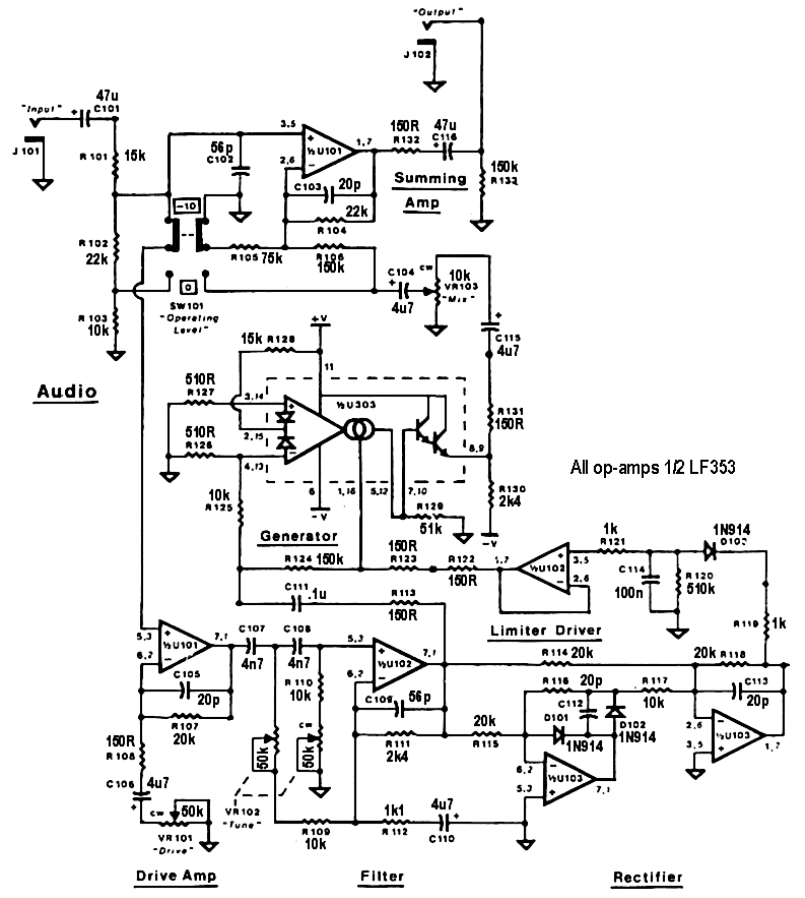
\includegraphics[height=2.5in]{Figures/exciter_circuit.png}
    \end{figure}
\end{frame}

\begin{frame}{Harmonic Exciter}
    \begin{figure}
        \centering
        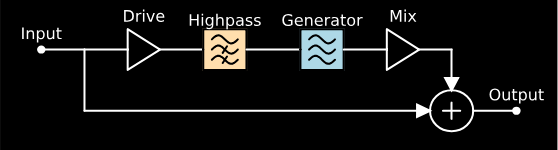
\includegraphics[width=4.25in]{../Exciter/Pics/Exciter_FullArch.png}
    \end{figure}
\end{frame}

\begin{frame}{Harmonic Exciter: Generator}
    \begin{figure}
        \centering
        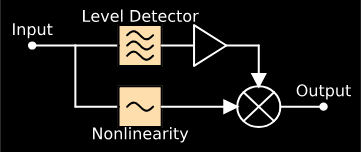
\includegraphics[width=4.25in]{../Exciter/Pics/Exciter_Arch.png}
    \end{figure}
\end{frame}

\begin{frame}{Harmonic Exciter: Level Detector}
    Rectifying nonlinearity \rightarrow LPF
    \begin{columns}
        \begin{column}{0.5\linewidth}
            \begin{figure}
                \centering
                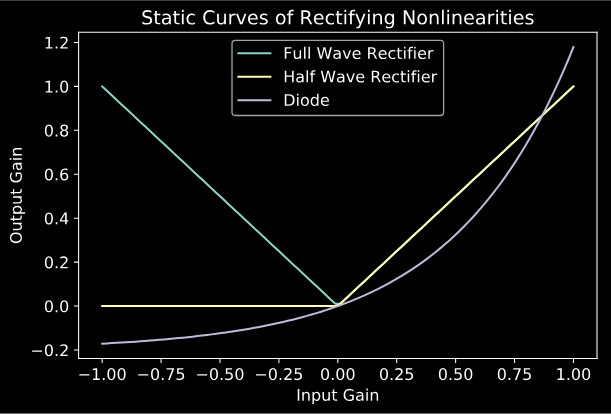
\includegraphics[width=2in]{../Exciter/Pics/rect_static}
            \end{figure}
        \end{column}
        \begin{column}{0.5\linewidth}
            \begin{figure}
                \centering
                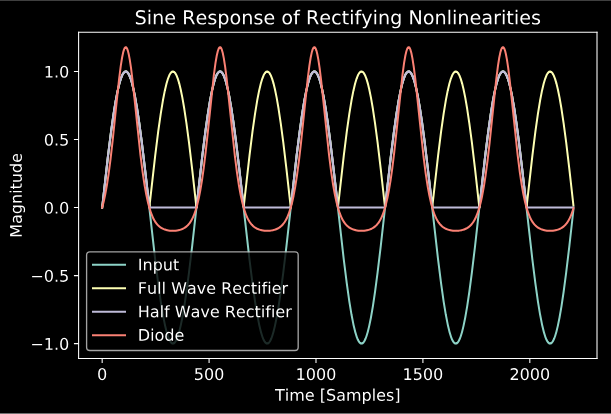
\includegraphics[width=2in]{../Exciter/Pics/rect_sine}
            \end{figure}
        \end{column}
    \end{columns}
\end{frame}

\begin{frame}{Harmonic Exciter: Level Detector}
    \begin{figure}
        \centering
        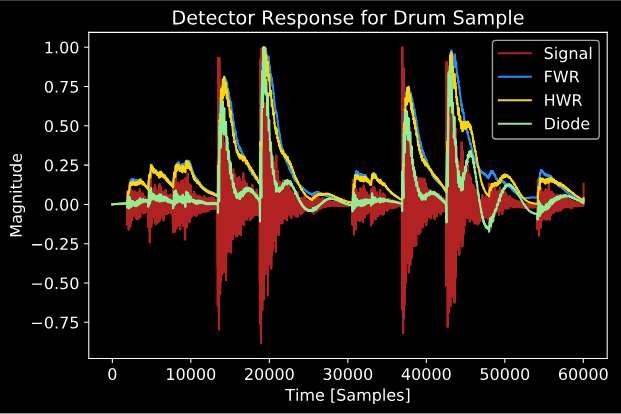
\includegraphics[height=2.5in]{../Exciter/Pics/Waveform_Detected.png}
    \end{figure}
\end{frame}

\begin{frame}{Harmonic Exciter: Nonlinearity}
    \begin{figure}
        \centering
        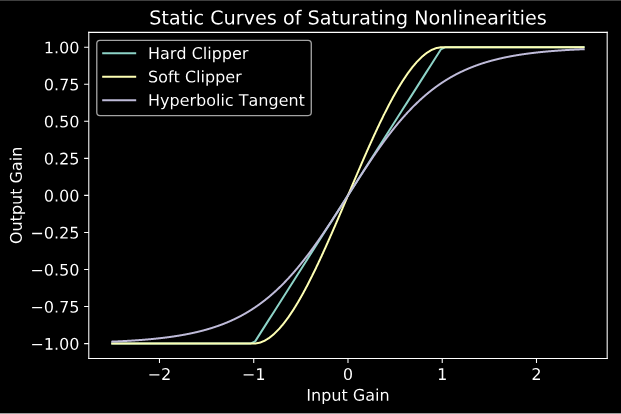
\includegraphics[height=2.5in]{../Exciter/Pics/saturating_static.png}
    \end{figure}
\end{frame}

\begin{frame}{Harmonic Exciter: Generator}
    \begin{figure}
        \centering
        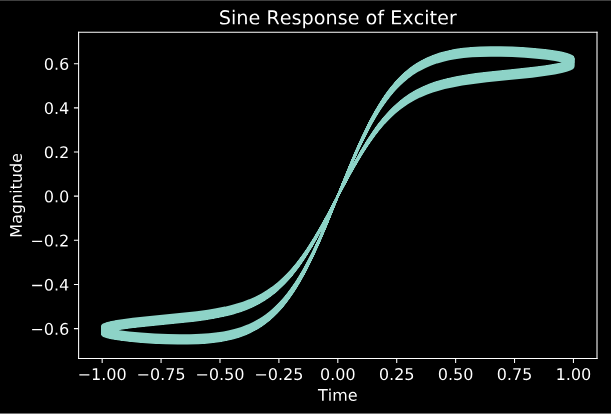
\includegraphics[height=2.5in]{../Exciter/Pics/exciter_static.png}
    \end{figure}
\end{frame}

\begin{frame}{Harmonic Exciter: Generator}
    \begin{figure}
        \centering
        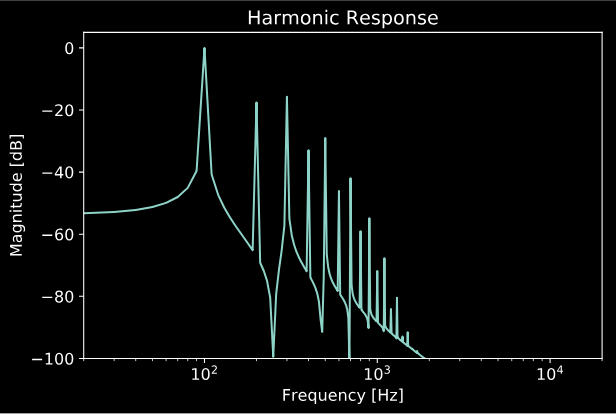
\includegraphics[height=2.5in]{../Exciter/Pics/exciter_harm.png}
    \end{figure}
\end{frame}

\begin{frame}
    \begin{centering}
        \vskip5ex plus 1filll
        {\usebeamerfont{title page title}\usebeamercolor[fg]{title page} Hysteresis\\[1.5ex]}
        \vskip0pt plus 1filll
    \end{centering}
\end{frame}

\begin{frame}{Hysteresis}
    \begin{columns}
        \begin{column}{0.5\linewidth}
            \begin{itemize}
                \item Stateful nonlinearity that describes magnetisation
                (magnetic tape, transformers, \dots)
                \item Also models processes in civil engineering,
                economics, and more
            \end{itemize}
        \end{column}
        \begin{column}{0.5\linewidth}
            \begin{figure}
                \centering
                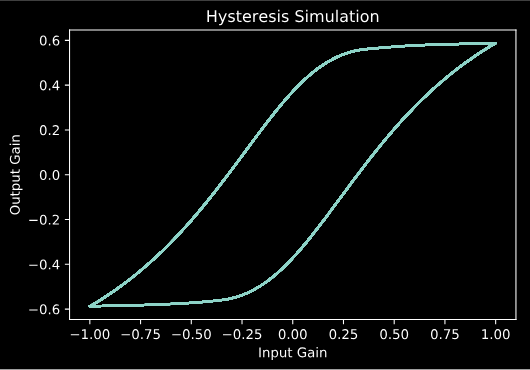
\includegraphics[width=2.5in]{../Hysteresis/Pics/First_Sim}
            \end{figure}
        \end{column}
    \end{columns}
\end{frame}

\begin{frame}{Hysteresis}
    Jiles-Atherton Hysteresis model\footcite{JilesAtherton1986}
    \begin{equation}
        \dot{y} = \frac{\frac{(1-c)\delta_y(SL(Q) - y)}{(1-c)\delta_xk - \alpha(SL(Q) - y)}\dot{x} + c \frac{S}{a} \dot{x} L'(Q)}{1 - c\alpha \frac{S}{a} L'(Q)}
    \end{equation}
    \begin{equation}
        Q(x,y) = \frac{x + \alpha y}{a}
    \end{equation}
    Langevin function:
    \vspace{-2ex}
    \begin{equation}
        L(x) = \coth(x) - \frac{1}{x}
    \end{equation}
\end{frame}

\begin{frame}{Hysteresis}
    Langevin function (and derivative)
    \begin{figure}
        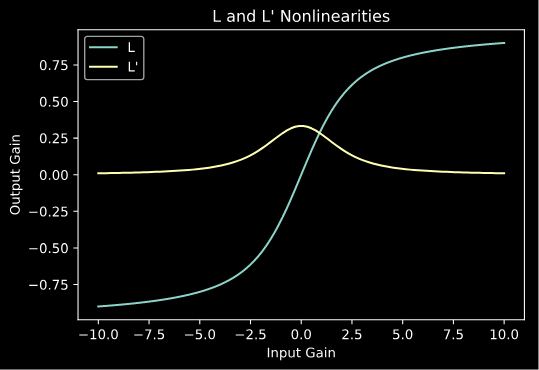
\includegraphics[height=2.5in]{../Hysteresis/Pics/LangevinPlot}
    \end{figure}
\end{frame}

\begin{frame}{Hysteresis}
    Digitize hysteresis model\footcite{Transformers_JA,DAFX-tape}
    \newline\newline
    Use $S, a, c$ as parameters
    \vspace{2ex}
    \begin{equation}
        \dot{y} = \frac{\frac{(1-c)\delta_y(SL(Q) - y)}{(1-c)\delta_xk - \alpha(SL(Q) - y)}\dot{x} + c \frac{S}{a} \dot{x} L'(Q)}{1 - c\alpha \frac{S}{a} L'(Q)}
    \end{equation}
\end{frame}

\begin{frame}{Hysteresis: Parameters}
    Saturation
    \begin{figure}
        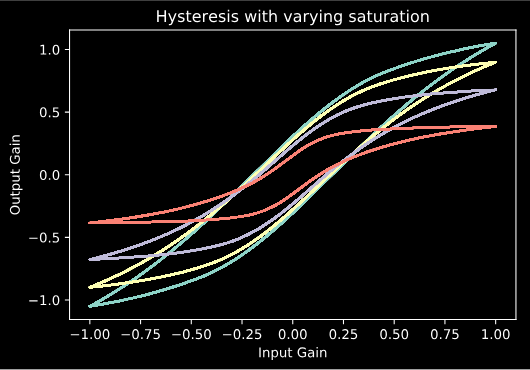
\includegraphics[height=2.5in]{../Hysteresis/Pics/Saturations}
    \end{figure}
\end{frame}

\begin{frame}{Hysteresis: Parameters}
    Drive
    \begin{figure}
        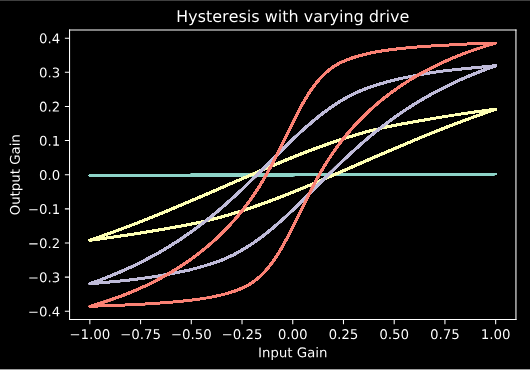
\includegraphics[height=2.5in]{../Hysteresis/Pics/Drive}
    \end{figure}
\end{frame}

\begin{frame}{Hysteresis: Parameters}
    Width
    \begin{figure}
        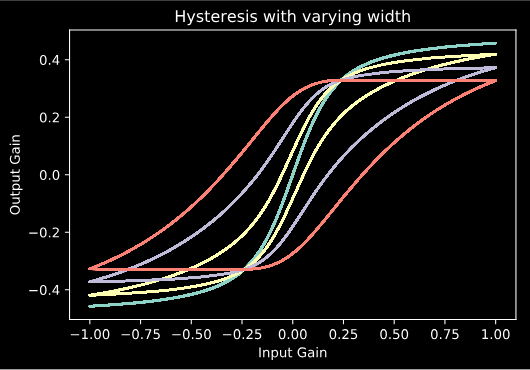
\includegraphics[height=2.5in]{../Hysteresis/Pics/Width}
    \end{figure}
\end{frame}

\begin{frame}{Hysteresis: Parameters}
    Width (with makeup gain)
    \begin{figure}
        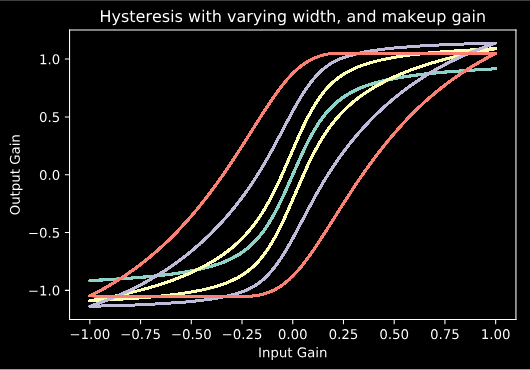
\includegraphics[height=2.5in]{../Hysteresis/Pics/Width_makeup}
    \end{figure}
\end{frame}

\begin{frame}{Hysteresis}
    \begin{columns}
        \begin{column}{0.5\linewidth}
            \begin{figure}
                \centering
                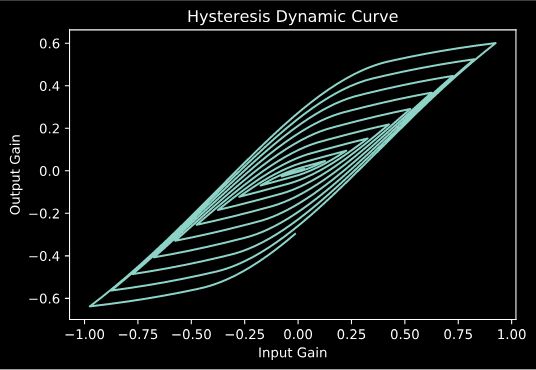
\includegraphics[width=2.75in]{../Hysteresis/Pics/Hysteresis_Dynamic}
            \end{figure}
        \end{column}
        \begin{column}{0.5\linewidth}
            \begin{figure}
                \centering
                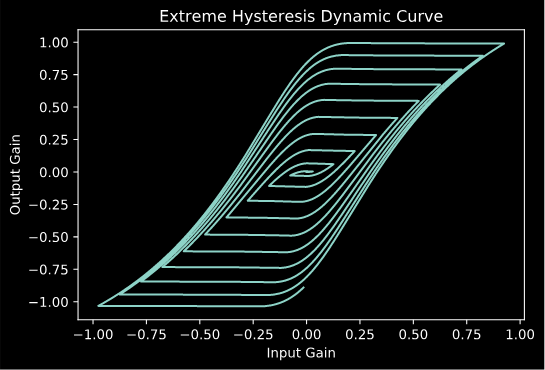
\includegraphics[width=2.75in]{../Hysteresis/Pics/Extreme_Hysteresis}
            \end{figure}
        \end{column}
    \end{columns}
\end{frame}

\begin{frame}
    \begin{centering}
        \vskip5ex plus 1filll
        {\usebeamerfont{title page title}\usebeamercolor[fg]{title page} Nonlinear Filters\\[1.5ex]}
        \vskip0pt plus 1filll
    \end{centering}
\end{frame}

\begin{frame}{Biquad Filter}
    Transposed Direct Form II
    \begin{figure}
        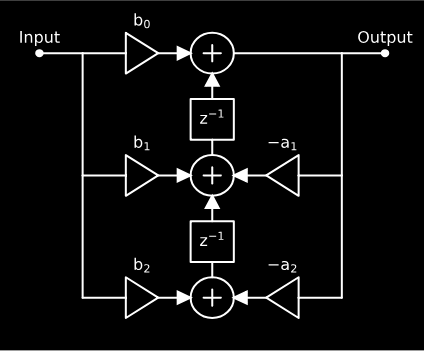
\includegraphics[height=2.5in]{../NonlinearBiquad/Pics/TDF-II.png}
    \end{figure}
\end{frame}

\begin{frame}{Biquad Filter}
    Difference equation:
    \begin{equation}
        y[n] = b_0 u[n] + b_1 u[n-1]
        + b_2 u[n-2] - a_1 y[n-1]
        - a_2 y[n-2]
    \end{equation}

    State space formulation:
    \begin{equation}
        \begin{bmatrix} x_1[n+1] \\ x_2[n+1] \\ y[n+1] \end{bmatrix} =
        \begin{bmatrix} 0& 1& -a_1\\ 0& 0& -a_2\\ 1& 0& 0 \end{bmatrix}
        \begin{bmatrix} x_1[n] \\ x_2[n] \\ y[n] \end{bmatrix}
        + \begin{bmatrix} b_1\\ b_2\\ b_0 \end{bmatrix} u[n]
    \end{equation}
\end{frame}

\begin{frame}{Nonlinear Biquad Filter}
    \begin{figure}
        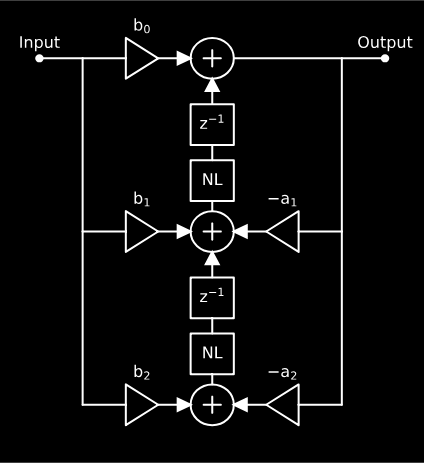
\includegraphics[height=2.5in]{../NonlinearBiquad/Pics/NL-TDF-II.png}
    \end{figure}
\end{frame}

\begin{frame}{Nonlinear Biquad Filter}
    Saturating nonlinearities \rightarrow nonlinear resonance
    \begin{figure}
        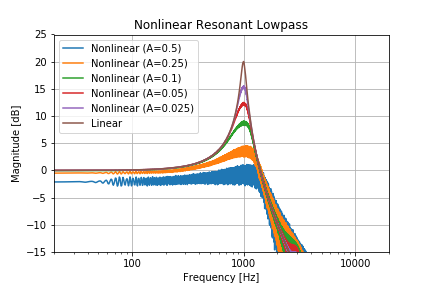
\includegraphics[height=2.5in]{../NonlinearBiquad/Pics/NL-LPF.png}
    \end{figure}
\end{frame}

\begin{frame}{Nonlinear Biquad Filter}
    Saturating nonlinearities \rightarrow nonlinear resonance
    \begin{figure}
        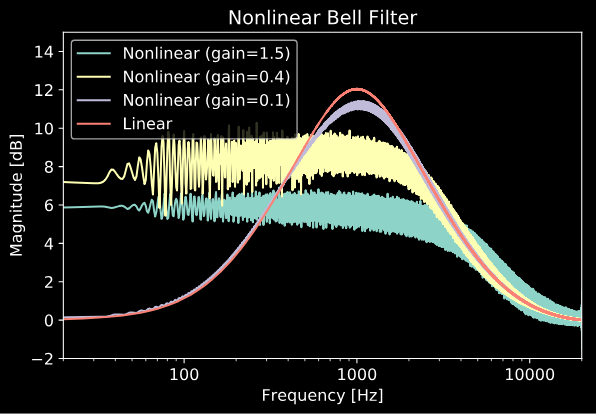
\includegraphics[height=2.5in]{../NonlinearBiquad/Pics/NL-Bell.png}
    \end{figure}
\end{frame}

\begin{frame}{Nonlinear Biquad Filter}
    Saturating nonlinearities \rightarrow nonlinear resonance
    \begin{figure}
        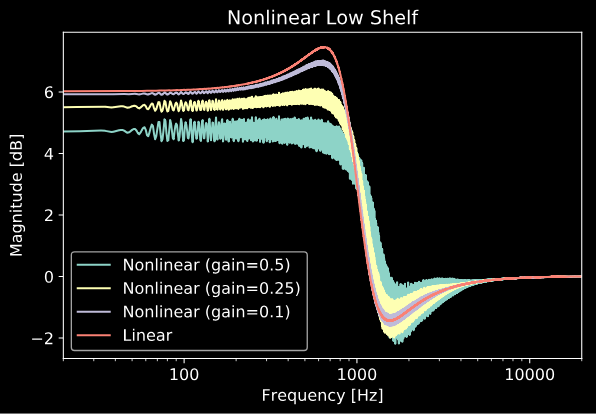
\includegraphics[height=2.5in]{../NonlinearBiquad/Pics/NL-LowShelf.png}
    \end{figure}
\end{frame}

\begin{frame}{Nonlinear Biquad Filter}
    Pole/zero movement
    \begin{figure}
        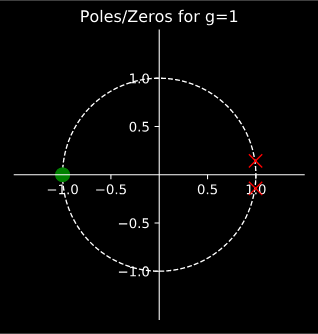
\includegraphics[width=1.33in]{../NonlinearBiquad/Pics/pz1.png}
        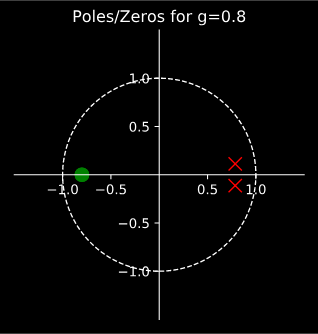
\includegraphics[width=1.33in]{../NonlinearBiquad/Pics/pz08.png}
        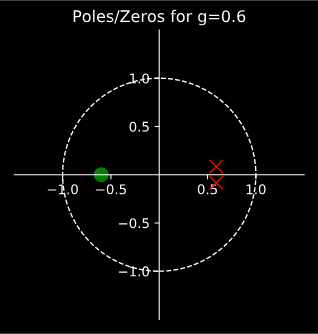
\includegraphics[width=1.33in]{../NonlinearBiquad/Pics/pz06.png}
        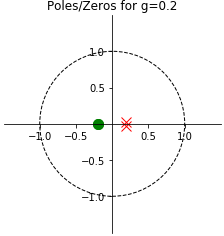
\includegraphics[width=1.33in]{../NonlinearBiquad/Pics/pz02.png}
    \end{figure}
\end{frame}

\begin{frame}{Nonlinear Feedback Filter}
    \begin{figure}
        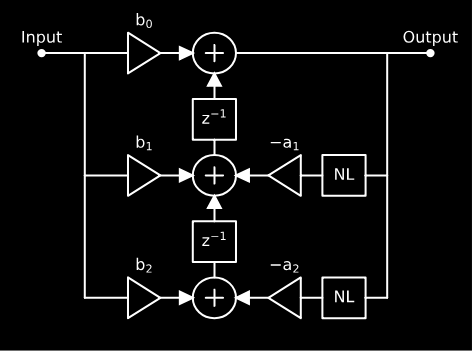
\includegraphics[height=2.5in]{../NonlinearFeedback/Pics/NL2-TDF-II.png}
    \end{figure}
\end{frame}

\begin{frame}{Nonlinear Feedback Filter}
    Saturating nonlinearity \rightarrow cutoff frequency modulation
    \begin{figure}
        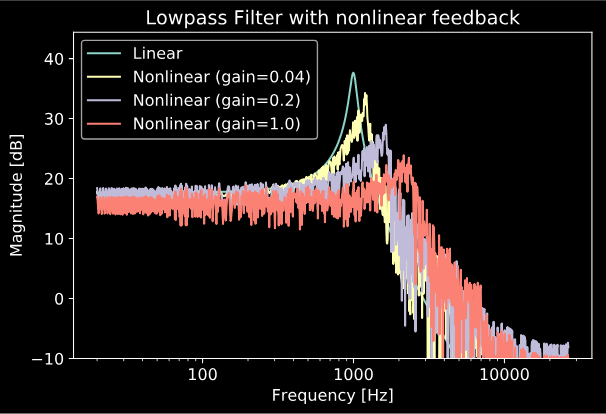
\includegraphics[height=2.5in]{../NonlinearFeedback/Pics/LPF-NL.png}
    \end{figure}
\end{frame}

\begin{frame}{Nonlinear Feedback Filter}
    Pole/zero movement
    \begin{figure}
        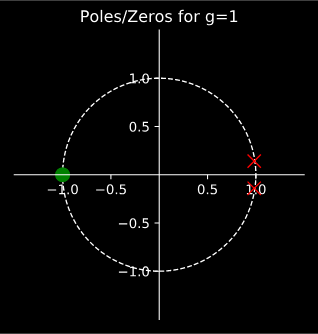
\includegraphics[width=1.33in]{../NonlinearFeedback/Pics/pz1.png}
        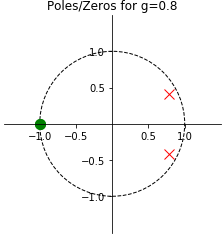
\includegraphics[width=1.33in]{../NonlinearFeedback/Pics/pz08.png}
        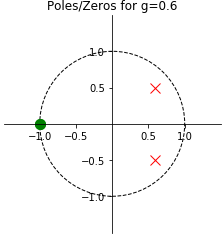
\includegraphics[width=1.33in]{../NonlinearFeedback/Pics/pz06.png}
        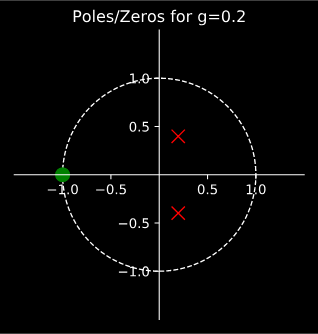
\includegraphics[width=1.33in]{../NonlinearFeedback/Pics/pz02.png}
    \end{figure}
\end{frame}

\begin{frame}{Nonlinear Biquad Stability}
    \textbf{Questions:}\newline\newline
    Can we guarantee that a nonlinear filter will be stable
    given that its linear corrolary is stable?
    \newline\newline
    For what subset of nonlinear functions is this guaranteed?
\end{frame}

\begin{frame}{Nonlinear Biquad Stability}
    Test case: saturating nonlinearity, $f_{NL} = \tanh(x)$ \rightarrow STABLE!
    \begin{figure}
        \includegraphics[height=2.5in]{Figures/nl_lpf_stable.png}
    \end{figure}
\end{frame}

\begin{frame}{Nonlinear Biquad Stability}
    Test case: full wave rectifier, $f_{NL} = 0.45 |x|$ \rightarrow UNSTABLE!
    \begin{figure}
        \includegraphics[height=2.5in]{Figures/nl_lpf_unstable.png}
    \end{figure}
\end{frame}

\begin{frame}{Nonlinear Biquad Stability}
    Test case: sine, $f_{NL} = \sin (x)$ \rightarrow STABLE!
    \begin{figure}
        \includegraphics[height=2.5in]{Figures/nl_lpf_sine.png}
    \end{figure}
\end{frame}

\begin{frame}{Lyapunov Stability\footcite{Lyapunov}}
    1. Form state space equation:
    \begin{equation}
        \mathbf{x}[n+1] = \mathbf{f}(\mathbf{x}[n])
    \end{equation}
    2. Find Jacobian $\mathbf{J}$ of $\mathbf{f}$
    \newline\newline
    3. If every element of $\mathbf{J}$ is less than 1
    at some operating point, the system is Lyapunov
    stable about that point.
\end{frame}

\begin{frame}{Nonlinear Biquad Stability}
    \begin{equation}
        \begin{bmatrix} x_1[n+1] \\ x_2[n+1] \\ y[n+1] \end{bmatrix} =
        \mathbf{h} \left( \begin{bmatrix} x_1[n] \\ x_2[n] \\ y[n] \end{bmatrix}
        \right) + \begin{bmatrix} b_1\\ b_2\\ b_0 \end{bmatrix} u[n]
    \end{equation}
    \vspace{3ex}
    \begin{equation}
        \begin{split}
            h_1(x_1[n], x_2[n], y[n]) =& f_{NL}(x_2[n]) - a_1y[n] \\
            h_2(x_1[n], x_2[n], y[n]) =& -a_2y[n] \\
            h_3(x_1[n], x_2[n], y[n]) =& f_{NL}(x_1[n])
        \end{split}
    \end{equation}
\end{frame}

\begin{frame}{Nonlinear Biquad Stability}
    \begin{equation}
        \mathbf{J} = \begin{bmatrix}
            0& f'_{NL}(x_2[n])& -a_1 \\
            0& 0& -a_2 \\
            f'_{NL}(x_1[n])& 0& 0
        \end{bmatrix}
    \end{equation}

    \vspace{3ex}

    Note that if $f'_{NL}$ does not exist at some point,
    the system is NOT stable at that point.
\end{frame}

\begin{frame}{Nonlinear Feedback Stability}
    \begin{equation}
        \begin{bmatrix} x_1[n+1] \\ x_2[n+1] \\ y[n+1] \end{bmatrix} =
        \mathbf{h} \left( \begin{bmatrix} x_1[n] \\ x_2[n] \\ y[n] \end{bmatrix}
        \right) + \begin{bmatrix} b_1\\ b_2\\ b_0 \end{bmatrix} u[n]
    \end{equation}
    \vspace{3ex}
    \begin{equation}
        \begin{split}
            h_1(x_1[n], x_2[n], y[n]) =& x_2[n] - a_1f_{NL}(y[n]) \\
            h_2(x_1[n], x_2[n], y[n]) =& -a_2f_{NL}(y[n]) \\
            h_3(x_1[n], x_2[n], y[n]) =& x_1[n]
        \end{split}
    \end{equation}
\end{frame}

\begin{frame}{Nonlinear Feedback Stability}
    \begin{equation}
        \mathbf{J} = \begin{bmatrix}
            0& 1& -a_1f'_{NL}(y[n]) \\
            0& 0& -a_2f'_{NL}(y[n]) \\
            1& 0& 0
        \end{bmatrix}
    \end{equation}
\end{frame}

\begin{frame}{Nonlinear Biquad Stability}
    General stability contstraint:
    \begin{equation}
        |f'_{NL}(x)| \leq 1
    \end{equation}
    \newline\newline
    \small
    Note: if the $f'_{NL}(x)$ does not exist, the filter is not guaranteed stable.
\end{frame}

\begin{frame}{Nonlinear Biquad Stability}
    If derivative doesn't exist at every point: use BLAMP\footcite{BLAMP}!
    \begin{figure}
        \includegraphics[height=2.2in]{Figures/blamp.png}
    \end{figure}
\end{frame}

\begin{frame}{Nonlinear Biquad Filter}
    Can we use this for analog modelling?
    \begin{figure}
        \includegraphics[height=2.5in]{../NonlinearBiquad/Pics/NL-LPF.png}
    \end{figure}
\end{frame}

\begin{frame}{Nonlinear Biquad Filter}
    Parameters: nonlinearities, input gain
    \begin{figure}
        \includegraphics[height=2.5in]{../NonlinearBiquad/Pics/50-Hz_Response.png}
    \end{figure}
\end{frame}

\begin{frame}{Nonlinear Biquad Filter}
    Modelling an overdriven Sallen-Key lowpass filter
    \begin{figure}
        \includegraphics[height=2.5in]{../NonlinearBiquad/Pics/Spice-Compare.png}
    \end{figure}
\end{frame}

\begin{frame}
    \begin{centering}
        \vskip5ex plus 1filll
        {\usebeamerfont{title page title}\usebeamercolor[fg]{title page} Wavefolding\\[1.5ex]}
        \vskip0pt plus 1filll
    \end{centering}
\end{frame}

\begin{frame}{Wavefolder}
    What is wavefolding?
    \begin{figure}
        \centering
        \includegraphics[width=4.5in]{Figures/wavefold.png}
    \end{figure}
\end{frame}

\begin{frame}{Wavefolder}
    Standard digital wavefolding:
    \vspace{2ex}
    \begin{columns}
        \begin{column}{0.5\linewidth}
            $f_{NL}(x) = sin(x)$
            \vspace{-3ex}
            \begin{figure}
                \includegraphics[height=2in]{../Wavefolder/Pics/sine_static}
            \end{figure}
        \end{column}
        \begin{column}{0.5\linewidth}
            $f_{NL}(x) = tri(x)$
            \vspace{-3ex}
            \begin{figure}
                \includegraphics[height=2in]{../Wavefolder/Pics/tri_static}
            \end{figure}
        \end{column}
    \end{columns}
\end{frame}

\begin{frame}{Wavefolder}
    Standard digital wavefolding:
    \begin{figure}
        \centering
        \includegraphics[height=2.5in]{../Wavefolder/Pics/simple_fold}
    \end{figure}
\end{frame}

\begin{frame}{Wavefolder}
    Saturating wavefolder:
    \begin{figure}
        \centering
        \includegraphics[width=4in]{../Wavefolder/Pics/sat_arch}
    \end{figure}
\end{frame}

\begin{frame}{Wavefolder}
    Saturating wavefolder:
    \begin{figure}
        \centering
        \includegraphics[height=2.5in]{../Wavefolder/Pics/sat_static}
    \end{figure}
\end{frame}

\begin{frame}{Wavefolder}
    Saturating wavefolder:
    \begin{figure}
        \centering
        \includegraphics[height=2.5in]{../Wavefolder/Pics/sat_wave}
    \end{figure}
\end{frame}

\begin{frame}{Wavefolder}
    Saturating wavefolder:
    \begin{figure}
        \centering
        \includegraphics[height=2.5in]{../Wavefolder/Pics/sat_wave_large}
    \end{figure}
\end{frame}

\begin{frame}{Wavefolder}
    Feedback wavefolder:
    \begin{figure}
        \centering
        \includegraphics[width=4in]{../Wavefolder/Pics/fb_arch}
    \end{figure}
\end{frame}

\begin{frame}{Wavefolder}
    Feedback wavefolder:
    \begin{figure}
        \centering
        \includegraphics[height=2.5in]{../Wavefolder/Pics/fb_dyn}
    \end{figure}
\end{frame}

% % \begin{frame}
    \begin{centering}
        \vskip5ex plus 1filll
        {\usebeamerfont{title page title}\usebeamercolor[fg]{title page} Nonlinear Allpass Filters\\[1.5ex]}
        \vskip0pt plus 1filll
    \end{centering}
\end{frame}

\begin{frame}
    \begin{centering}
        \vskip5ex plus 1filll
        {\usebeamerfont{title page title}\usebeamercolor[fg]{title page} Subharmonics\\[1.5ex]}
        \vskip0pt plus 1filll
    \end{centering}
\end{frame}

\begin{frame}{Subharmonics: Motivation}
    Most nonlinear audio effects add higher harmonics to the signal.
    \newline\newline
    What if we want lower harmonics \dots
\end{frame}

\begin{frame}{Subharmonics}
    Goals:
    \vspace{3ex}
    \begin{itemize}
        \item Generate subharmonic content
        \item Avoid circuit modelling
        \item Avoid relying on high-quality pitch detection
    \end{itemize}
\end{frame}

\begin{frame}{Subharmonics}
    Step 1: Detect when the input signal switches directions
    \begin{figure}
        \centering
        \includegraphics[height=2.5in]{../Subharmonics/Pics/rise_fall.png}
    \end{figure}
\end{frame}

\begin{frame}{Subharmonics}
    Step 2: Flip detector signal every \emph{other} time
    \begin{figure}
        \centering
        \includegraphics[height=2.25in]{../Subharmonics/Pics/half_square.png}
    \end{figure}
    Result: half-frequency square wave!
\end{frame}

\begin{frame}{Subharmonics}
    Step 3: Lowpass Filter
    \begin{figure}
        \centering
        \includegraphics[height=2.5in]{../Subharmonics/Pics/half_sine.png}
    \end{figure}
\end{frame}

\begin{frame}{Subharmonics}
    \begin{figure}
        \centering
        \includegraphics[height=2.5in]{../Subharmonics/Pics/freq_compare.png}
    \end{figure}
\end{frame}

\begin{frame}{Subharmonics}
    Step 4: Apply level detector
    \begin{figure}
        \centering
        \includegraphics[height=2.5in]{../Subharmonics/Pics/LD_example.png}
    \end{figure}
\end{frame}

\begin{frame}{Subharmonics}
    \begin{figure}
        \centering
        \includegraphics[width=4.5in]{../Subharmonics/Pics/full_arch.png}
    \end{figure}
\end{frame}

\begin{frame}
    \begin{centering}
        \vskip5ex plus 1filll
        {\usebeamerfont{title page title}\usebeamercolor[fg]{title page} Gated Recurrent Distortion\\[1.5ex]}
        \vskip0pt plus 1filll
    \end{centering}
\end{frame}

\begin{frame}{Gated Recurrent Distortion}
    Gated Recurrent Unit:
    \vspace{3ex}
    \begin{itemize}
        \item Building block for recurrent neural networks \footcite{gru_original}
        \item Here we examine a variation: ``minimal gated unit'' \footcite{minimal-gated-unit}
    \end{itemize}
\end{frame}

\begin{frame}{Gated Recurrent Distortion}
    \begin{equation}
        \begin{split}
            \Gamma_f &= \sigma (W_f x[n] + U_f y[n-1] + b_f) \\
            y[n] &= \Gamma_f y[n-1] + (1 - \Gamma_f) \tanh (W_h x[n] + U_h \Gamma_f y[n-1] + b_h)
        \end{split}
    \end{equation}
    \vspace{3ex}
    \begin{equation}
        \sigma(x) = \frac{1}{1 + e^{-x}}
        \label{eq:sigmoid}
    \end{equation}
\end{frame}

\begin{frame}{Gated Recurrent Distortion}
    \begin{columns}
        \begin{column}{0.5\linewidth}
            \begin{figure}
                \includegraphics[height=2in]{../GatedRecurrentDistortion/Pics/sigmoid}
            \end{figure}
        \end{column}
        \begin{column}{0.5\linewidth}
            \begin{figure}
                \includegraphics[height=2in]{../GatedRecurrentDistortion/Pics/tanh}
            \end{figure}
        \end{column}
    \end{columns}
\end{frame}

\begin{frame}{Gated Recurrent Distortion}
    \begin{figure}
        \centering
        \includegraphics[height=2.5in]{../GatedRecurrentDistortion/Pics/gru_arch}
    \end{figure}
\end{frame}

\begin{frame}{Gated Recurrent Distortion: Parameters}
    \begin{figure}
        \centering
        \includegraphics[height=2.5in]{../GatedRecurrentDistortion/Pics/wh}
    \end{figure}
\end{frame}

\begin{frame}{Gated Recurrent Distortion: Parameters}
    \begin{columns}
        \begin{column}{0.5\linewidth}
            \begin{figure}
                \centering
                \includegraphics[width=2.75in]{../GatedRecurrentDistortion/Pics/wf}
            \end{figure}
        \end{column}
        \begin{column}{0.5\linewidth}
            \begin{figure}
                \centering
                \includegraphics[width=2.75in]{../GatedRecurrentDistortion/Pics/uf}
            \end{figure}
        \end{column}
    \end{columns}
\end{frame}

\begin{frame}{Gated Recurrent Distortion: Parameters}
    \begin{columns}
        \begin{column}{0.5\linewidth}
            \begin{figure}
                \centering
                \includegraphics[width=2.75in]{../GatedRecurrentDistortion/Pics/uh}
            \end{figure}
        \end{column}
        \begin{column}{0.5\linewidth}
            \begin{figure}
                \centering
                \includegraphics[width=2.75in]{../GatedRecurrentDistortion/Pics/bf}
            \end{figure}
        \end{column}
    \end{columns}
\end{frame}

\begin{frame}{Gated Recurrent Distortion: Harmonic Response}
    \begin{columns}
        \begin{column}{0.5\linewidth}
            \begin{figure}
                \centering
                \includegraphics[width=2.75in]{../GatedRecurrentDistortion/Pics/odd_harm}
            \end{figure}
        \end{column}
        \begin{column}{0.5\linewidth}
            \begin{figure}
                \centering
                \includegraphics[width=2.75in]{../GatedRecurrentDistortion/Pics/all_harm}
            \end{figure}
        \end{column}
    \end{columns}
\end{frame}

\begin{frame}
    \begin{centering}
        \vskip5ex plus 1filll
        {\usebeamerfont{title page title}\usebeamercolor[fg]{title page} Conclusion\\[1.5ex]}
        \vskip0pt plus 1filll
    \end{centering}
\end{frame}

\begin{frame}{Goals}
    \begin{itemize}
        \item Tools for musicians/mixing engineeers
        \item Inspiration/explanations for audio effect makers
        \item A academic paper (or two)
    \end{itemize}
\end{frame}

\begin{frame}{Presentation}
    Audio plugins (VST/AU)
    \vspace{1ex}
    \begin{figure}
        \centering
        \includegraphics[height=2.5in]{Figures/GRU_screenshot}
    \end{figure}
\end{frame}

\begin{frame}{Presentation}
    Medium articles
    \vspace{1ex}
    \begin{figure}
        \centering
        \includegraphics[height=2.5in]{Figures/medium}
    \end{figure}
\end{frame}

\begin{frame}{Presentation}
    Papers
    \vspace{-1ex}
    \begin{columns}
        \begin{column}{0.5\linewidth}
            \hspace{-1ex}
            \begin{figure}
                \centering
                \includegraphics[height=2.4in,width=2.3in]{Figures/paper1}
            \end{figure}
        \end{column}
        \begin{column}{0.5\linewidth}
            \begin{figure}
                \centering
                \includegraphics[height=2.4in,width=2.3in]{Figures/paper2}
            \end{figure}
        \end{column}
    \end{columns}
\end{frame}

\begin{frame}{Presentation}
    Links:
    \begin{itemize}
        \item \url{https://github.com/jatinchowdhury18/ComplexNonlinearities}
        \item \url{https://medium.com/@jatinchowdhury18}
    \end{itemize}
\end{frame}

\begin{frame}{}
    \begin{centering}
        \vskip5ex plus 1filll
        {\usebeamerfont{title page title}\usebeamercolor[fg]{title page} Thank you!\\[1.5ex]}
        \vskip0pt plus 1filll
    \end{centering}
\end{frame}




\end{document}
